%%%%%% Run at command line, run
%%%%%% xelatex grad-sample.tex 
%%%%%% for a few times to generate the output pdf file
\documentclass[12pt,oneside,openright,a4paper]{cpe-thai-project}

\usepackage{caption}

\defaultfontfeatures{Mapping=tex-text,Scale=1.23,LetterSpace=0.0}
\setmainfont[Scale=1.23,LetterSpace=0,WordSpace=1.0,FakeStretch=1.0]{TH Sarabun New}
%\setmathfont(Digits)[Scale=1.0,LetterSpace=0,FakeStretch=1.0]{Times New Roman}


%%%%%%%%%%%%%%%%%%%%%%%%%%%%%%%%%%%%%%%%%%%%%%%%%%%%%%%%%%%%%%%%%%%
% Customize below to suit your needs 
% The ones that are optional can be left blank. 
%%%%%%%%%%%%%%%%%%%%%%%%%%%%%%%%%%%%%%%%%%%%%%%%%%%%%%%%%%%%%%%%%%%
% First line of title
\def\disstitleone{Your Art Painter}   
% Second line of title
\def\disstitletwo{(จิตรกรผู้สร้างศิลปะของคุณ)}   
% Your first name and lastname
\def\dissauthor{Mr. Nawarit Longkhum}   % 1st member
%%% Put other group member names here ..
\def\dissauthortwo{Ms. Pataraphorn Tanutsiriteeradet​}   % 2nd member (optional)
\def\dissauthorthree{Ms. Sukasama   Chitakson}   % 3rd member (optional)


% The degree that you're persuing..
\def\dissdegree{Bachelor of Engineering} % Name of the degree
\def\dissdegreeabrev{B.Eng} % Abbreviation of the degree
\def\dissyear{2020}                   % Year of submission
\def\thaidissyear{2563}               % Year of submission (B.E.)

%%%%%%%%%%%%%%%%%%%%%%%%%%%%%%%%%%%%%%%%%%%%
% Your project and independent study committee..
%%%%%%%%%%%%%%%%%%%%%%%%%%%%%%%%%%%%%%%%%%%%
\def\dissadvisor{Assoc.Prof. My main advisor name , Ph.D.}  % Advisor
%%% Leave it empty if you have no Co-advisor
\def\disscoadvisor{Assoc.Prof. My Co-advisor name, Ph.D.}  % Co-advisor
\def\disscommitteetwo{Asst.Prof. Committee2, Ph.D.}  % 3rd committee member (optional)
\def\disscommitteethree{Asst.Prof. Committee3, Ph.D.}   % 4th committee member (optional) 
\def\disscommitteefour{}    % 5th committee member (optional) 

\def\worktype{Project} %%  Project or Independent study
\def\disscredit{3}   %% 3 credits or 6 credits


\def\fieldofstudy{Computer Engineering} 
\def\department{Computer Engineering} 
\def\faculty{Engineering}

\def\thaifieldofstudy{วิศวกรรมคอมพิวเตอร์} 
\def\thaidepartment{วิศวกรรมคอมพิวเตอร์} 
\def\thaifaculty{วิศวกรรมศาสตร์}
 
\def\appendixnames{Appendix} %%% Appendices or Appendix

\def\thaiworktype{ปริญญานิพนธ์} %  Project or research project % 
\def\thaidisstitleone{หัวข้อปริญญานิพนธ์บรรทัดแรก}
\def\thaidisstitletwo{หัวข้อปริญญานิพนธ์บรรทัดสอง}
\def\thaidissauthor{นายสมศักดิ์ คอมพิวเตอร์}
\def\thaidissauthortwo{นางสาวสมศรี คอมพิวเตอร์2} %Optional
\def\thaidissauthorthree{นางสาวสมปอง คอมพิวเตอร์3} %Optional

\def\thaidissadvisor{รศ.ดร.ที่ปรึกษา วิทยานิพนธ์}
%% Leave this empty if you have no co-advisor
\def\thaidisscoadvisor{รศ.ดร.ที่ปรึกษา วิทยานิพนธ์ร่วม} %Optional
\def\thaidissdegree{วิศวกรรมศาสตรบัณฑิต}

% Change the line spacing here...
\linespread{1.15}

%%%%%%%%%%%%%%%%%%%%%%%%%%%%%%%%%%%%%%%%%%%%%%%%%%%%%%%%%%%%%%%%
% End of personal customization.  Do not modify from this part 
% to \begin{document} unless you know what you are doing...
%%%%%%%%%%%%%%%%%%%%%%%%%%%%%%%%%%%%%%%%%%%%%%%%%%%%%%%%%%%%%%%%


%%%%%%%%%%%% Dissertation style %%%%%%%%%%%
%\linespread{1.6} % Double-spaced  
%%\oddsidemargin    0.5in
%%\evensidemargin   0.5in
%%%%%%%%%%%%%%%%%%%%%%%%%%%%%%%%%%%%%%%%%%%
%\renewcommand{\subfigtopskip}{10pt}
%\renewcommand{\subfigbottomskip}{-5pt} 
%\renewcommand{\subfigcapskip}{-6pt} %vertical space between caption
%                                    %and figure.
%\renewcommand{\subfigcapmargin}{0pt}

\renewcommand{\topfraction}{0.85}
\renewcommand{\textfraction}{0.1}
\newcommand{\source}[1]{\caption*{Source: {#1}} }

\newtheorem{theorem}{Theorem}
\newtheorem{lemma}{Lemma}
\newtheorem{corollary}{Corollary}

\def\QED{\mbox{\rule[0pt]{1.5ex}{1.5ex}}}
\def\proof{\noindent\hspace{2em}{\itshape Proof: }}
\def\endproof{\hspace*{\fill}~\QED\par\endtrivlist\unskip}
%\newenvironment{proof}{{\sc Proof:}}{~\hfill \blacksquare}
%% The hyperref package redefines the \appendix. This one 
%% is from the dissertation.cls
%\def\appendix#1{\iffirstappendix \appendixcover \firstappendixfalse \fi \chapter{#1}}
%\renewcommand{\arraystretch}{0.8}
%%%%%%%%%%%%%%%%%%%%%%%%%%%%%%%%%%%%%%%%%%%%%%%%%%%%%%%%%%%%%%%%
%%%%%%%%%%%%%%%%%%%%%%%%%%%%%%%%%%%%%%%%%%%%%%%%%%%%%%%%%%%%%%%%
\begin{document}

\makesignaturepage 

%%%%%%%%%%%%%%%%%%%%%%%%%%%%%%%%%%%%%%%%%%%%%%%%%%%%%%%%%%%%%%
%%%%%%%%%%%%%%%%%%%%%% English abstract %%%%%%%%%%%%%%%%%%%%%%%
%%%%%%%%%%%%%%%%%%%%%%%%%%%%%%%%%%%%%%%%%%%%%%%%%%%%%%%%%%%%%%
\abstract

In a multihop ad hoc network, the interference among nodes is
  reduced to maximize the throughput by using a smallest transmission
  range that still preserve the network connectivity. However, most
  existing works on transmission range control focus on the
  connectivity but lack of results on the throughput performance. This
  paper analyzes the per-node saturated throughput of an IEEE 802.11b
  multihop ad hoc network with a uniform transmission range. Compared
  to simulation, our model can accurately predict the per-node
  throughput.  The results show that the maximum achievable per-node
  throughput can be as low as 11\% of the channel capacity in a normal
  set of $\alpha$ operating parameters independent of node density. However, if
  the network connectivity is considered, the obtainable throughput
  will reduce by as many as 43\% of the maximum throughput. 

\begin{flushleft}
\begin{tabular*}{\textwidth}{@{}lp{0.8\textwidth}}
\textbf{Keywords}: & Multihop ad hoc networks / Topology control / Single-Hop Throughput
\end{tabular*}
\end{flushleft}
\endabstract

%%%%%%%%%%%%%%%%%%%%%%%%%%%%%%%%%%%%%%%%%%%%%%%%%%%%%%%%%%%%%%
%%%%%%%%%% Thai abstract here %%%%%%%%%%%%%%%%%%%%%%%%%%%%%%%%%
%%%%%%%%%%%%%%%%%%%%%%%%%%%%%%%%%%%%%%%%%%%%%%%%%%%%%%%%%%%%%%
{\newfontfamily\thaifont{TH Sarabun New:script=thai}[Scale=1.3]
\XeTeXlinebreaklocale "th_TH"	
\thaifont
\thaiabstract

การวิจัยครั้งนี้มีวัตถุประสงค์  เพื่อศึกษาความพึงพอใจในการให้บริการงานทั่วไปของสานักวิชา พื้นฐานและภาษา เพื่อเปรียบเทียบระดับความพึงพอใจต่อการให้บริการงาน ทั่วไปของสานักวิชาพื้นฐานและภาษา ของนักศึกษาที่มาใช้บริการสานักวิชาพื้นฐานและภาษา สถาบัน เทคโนโลยีไทย-ญี่ปุ่น จาแนกตามเพศ คณะ และชั้นปีที่ศึกษา เพื่อศึกษาปัญหาและข้อเสนอแนะของ นักศึกษามาเป็นแนวทางในการพัฒนาและปรับปรุงการให้บริการของสานักวิชาพื้นฐานและภาษา

\begin{flushleft}
\begin{tabular*}{\textwidth}{@{}lp{0.8\textwidth}}
 & \\

\textbf{คำสำคัญ}: & การชุบเคลือบด้วยไฟฟ้า / การชุบเคลือบผิวเหล็ก /  เคลือบผิวรังสี
\end{tabular*}
\end{flushleft}
\endabstract
}

%%%%%%%%%%%%%%%%%%%%%%%%%%%%%%%%%%%%%%%%%%%%%%%%%%%%%%%%%%%%
%%%%%%%%%%%%%%%%%%%%%%% Acknowledgments %%%%%%%%%%%%%%%%%%%%
%%%%%%%%%%%%%%%%%%%%%%%%%%%%%%%%%%%%%%%%%%%%%%%%%%%%%%%%%%%%
\preface
ขอบคุณอาจารย์ที่ปรึกษา กรรมการ พ่อแม่พี่น้อง และเพื่อนๆ คนที่ช่วยให้งานสำเร็จ ตามต้องการ

%%%%%%%%%%%%%%%%%%%%%%%%%%%%%%%%%%%%%%%%%%%%%%%%%%%%%%%%%%%%%
%%%%%%%%%%%%%%%% ToC, List of figures/tables %%%%%%%%%%%%%%%%
%%%%%%%%%%%%%%%%%%%%%%%%%%%%%%%%%%%%%%%%%%%%%%%%%%%%%%%%%%%%%
% The three commands below automatically generate the table 
% of content, list of tables and list of figures
\tableofcontents                    
\listoftables
\listoffigures                      

%%%%%%%%%%%%%%%%%%%%%%%%%%%%%%%%%%%%%%%%%%%%%%%%%%%%%%%%%%%%%%
%%%%%%%%%%%%%%%%%%%%% List of symbols page %%%%%%%%%%%%%%%%%%%
%%%%%%%%%%%%%%%%%%%%%%%%%%%%%%%%%%%%%%%%%%%%%%%%%%%%%%%%%%%%%%
% You have to add this manually..
\listofsymbols
\begin{flushleft}
\begin{tabular}{@{}p{0.07\textwidth}p{0.7\textwidth}p{0.1\textwidth}}
\textbf{SYMBOL}  & & \textbf{UNIT} \\[0.2cm]
$\alpha$ & Test variable\hfill & m$^2$ \\
$\lambda$ & Interarival rate\hfill &  jobs/second\\
$\mu$ & Service rate\hfill & jobs/second\\
\end{tabular}
\end{flushleft}
%%%%%%%%%%%%%%%%%%%%%%%%%%%%%%%%%%%%%%%%%%%%%%%%%%%%%%%%%%%%%%
%%%%%%%%%%%%%%%%%%%%% List of vocabs & terms %%%%%%%%%%%%%%%%%
%%%%%%%%%%%%%%%%%%%%%%%%%%%%%%%%%%%%%%%%%%%%%%%%%%%%%%%%%%%%%%
% You also have to add this manually..
\listofvocab
\begin{flushleft}
\begin{tabular}{@{}p{1in}@{=\extracolsep{0.5in}}l}
ABC & Adaptive Bandwidth Control \\
MANET & Mobile Ad Hoc Network 
\end{tabular}
\end{flushleft}

%\setlength{\parskip}{1.2mm}

%%%%%%%%%%%%%%%%%%%%%%%%%%%%%%%%%%%%%%%%%%%%%%%%%%%%%%%%%%%%%%%
%%%%%%%%%%%%%%%%%%%%%%%% Main body %%%%%%%%%%%%%%%%%%%%%%%%%%%%
%%%%%%%%%%%%%%%%%%%%%%%%%%%%%%%%%%%%%%%%%%%%%%%%%%%%%%%%%%%%%%%


\chapter{บทนำ}






\section{ที่มาและความสำคัญ}

\par\setlength{\parindent}{5ex}กว่า 5,000 ปีมาแล้ว ตั้งแต่ยุคก่อนประวัติศาตร์ ที่มนุษย์รู้จักการวาดรูป โดยเริ่มแรกมนุษย์วาดภาพครั้งแรกโดยการขีดขูดบนผนังถ้ำหรือเพิงพา โดยรูปภาพที่วาดออกมาจะเป็นภาพคน สัตว์ หรือการล่าสัตว์ ซึ่งแสดงให้เห็นถึงชีวิตความเป็นอยู่ของคนในยุคสมัยนั้น และหลังจากนั้นมนุษย์ได้มีการพัฒนาการวาดรูปอยู่ตลอดเวลา จากการวาดรูปตามผนังถ้ำ ตามผนังโบสถ์ หรือราชวังที่สำคัญต่างๆ จนมาเป็นวาดรูปตามผืนผ้า ตลอดจนมาเป็นในกระดาษ ภาพวาดนั้นนอกจะวาดเพื่อถ่ายถอดเรื่องราวในอดีตแล้ว ยังแสดงให้เห็นถึงเอกลักษณ์ของศิลปินอีกด้วย ซึ่งศิลปินของโลกทางตะวันตกและตะวันออกก็มีลักษณะที่แตกต่างกัน และในแต่ละประเทศหรือศิลปินแต่ละท่านก็จะมีเทคนิตวิธีการวาดที่ไม่เหมือนกัน ศิลปินไทยที่มีชื่อในการวาดภาพ เช่น อ.เฉลิมชัย โฆษิตพิพัฒน์ อ.ชลูด นิ่มเสมอ และอ.จักรพันธุ์ โปษยกฤต เป็นต้น style ในการวาดของศิลปินแต่ละท่านก็มีความแตกต่างกัน ทำให้ผู้คนชื่นชอบงานของท่าน และอยากมีภาพที่มีสไตล์แบบนั้น 
\par\setlength{\parindent}{5ex}จนกระทั่งปี 2015 Gatys et al. ได้ตีพิมพ์ผลงาน A Neural Algorithm of Artistic Style ซึ่งเป็นการศึกษาเกี่ยวกับการนำเอาภาพ style ที่มีชื่อเสียงไปรวมกับภาพวิวเมือง Tubingen, ประเทศเยอรมัน โดยใช้แนวคิดของ Convolutional Neural Network (CNN)  ได้สำเร็จ ออกมาเป็นรูปภาพที่เป็นรูปภาพวิวเมือง Tubingen แต่ได้ใช้เทคนิคการวาดรูปจากศิลปินชื่อดัง ทำให้ภาพที่ได้มาใหม่นั้นดูเหมือนศิลปินที่เสียชีวิตไปแล้วกลับมาวาดรูปขึ้นใหม่ จากความสำเร็จครั้งนั้น ส่งผลให้มีคนจำนวนมากสนใจในการทำ Neural Style Transfer (NST) และ CNN มากขึ้น
\par\setlength{\parindent}{5ex}ดังนั้นทางคณะผู้จัดทำจึงต้องการศึกษาวิธีการทำ Neural Style Transfer ที่มี Convolutional Neural Network (CNN) เป็นทฤษฎีเบื้องหลัง และนำความรู้ที่ได้มาพัฒนาโมเดลที่สามารถทำ Neural Style Transfer รูปที่วาดโดยอ.จักรพันธุ์ โปษยกฤตและอ.ชลูด นิ่มเสมอซึ่งเป็นศิลปินไทยได้ อีกทั้งเพื่อเพื่อพัฒนา web application ที่มาสามารถสร้างรูปภาพจากที่มีลักษณะของศิลปินผสมผสานได้

\section{ประเภทของโครงงาน}
\par\setlength{\parindent}{5ex}นําเสนอความต้องการของผู้มีส่วนได้ส่วนเสียเฉพาะกลุ่ม ผลิตภัณฑ์ทางการค้าที่มีศักยภาพ และ เว็บแอปพลิเคชันสำหรับคอมพิวเตอร์

\section{วิธีการนำเสนอ}
\par\setlength{\parindent}{5ex}ในการบรรลุวัตถุประสงค์ของโครงการนั้น ใช้วิธีการดังต่อไปนี้
\begin{enumerate}
\item เตรียมชุดข้อมูลเพื่อนำไปใช้ train โมเดล\par\setlength{\parindent}{5ex}รวบรวมรูปภาพที่สร้างจากศิลปินที่มีชื่อเสียงและลักษณะภาพสามารถบอกได้ถึงเอกลักษณ์ของศิลปินท่านนั้นได้ โดยทางผู้จัดทำได้รวบรวมรูปภาพของศิลปิน จำนวน 2 ท่านได้แก่ อ.จักรพันธุ์ โปษยกฤษ และ อ. ชลูด นิ่มเสมอ เพื่อใช้เป็น style image และรวบรวมรูปภาพคนหรือสัตว์ทั่ว ๆ ไป เพื่อใช้เป็น content image
\item จัดการรูปภาพให้อยู่ในรูปแบบที่ใช้ในโมเดล (Data preprocessing)\par\setlength{\parindent}{5ex} จัดการรูปภาพทั้ง style image และ content image ในเหมาะสมโดยทำการเพิ่มความละเอียด เพิ่มความคมชัด เป็นต้นและแปลงรูปภาพให้อยู่ในลักษณะที่สามารถใช้กับโมเดลได้ คือ ขนาด 224*224 พิกเซล
\item สร้างโมเดลและปรับค่า parameter \par\setlength{\parindent}{5ex}นำโมเดลของ VGGNet ที่มีอัลกอริทึม convolutional neural network (CNN) อยู่เบื้องหลังมาใช้เพื่อค้นหารูปแบบและลักษณะเด่นของภาพออกมา (Feature Extraction) จากนั้นเอาลักษณะเด่นของ style image และ content image มารวมกันเพื่อสร้างรูปภาพใหม่ที่เป็นแบบ content image แต่มีลักษณะของ style  image ผสมผสานเข้าด้วยกัน โดยปรับค่า weight และ bias จนได้โมเดลที่มีค่า loss function เหมาะสม
\item นำรูปภาพที่สร้างจากศิลปินท่านอื่นหรือ style image รูปอื่น ๆ มา train ร่วมกับ content image เดิม และปรับค่าต่าง ๆ ให้โมเดลสามารถทำงานกับรูปอื่นได้ทั่วไป
\item ทดลองใช้งานโมเดล โดยนำรูปภาพคนหรือสัตว์ รูปอื่น ๆ มาใช้งานโมเดลแล้วแก้ไขข้อผิดพลาดและพัฒนาให้โมเดลดียิ่งขึ้นจากเดิม
\item สร้าง Web Application ตามที่ได้ออกแบบไว้
\end{enumerate}

\newpage

\section{วัตถุประสงค์ของโครงการ}
\begin{enumerate}
  \item	เพื่อศึกษาการทำ Neural Style Transfer ที่มี Convolutional Neural Network (CNN) เป็นทฤษฎีเบื้องหลัง
  \item เพื่อพัฒนาโมเดลที่สามารถทำ Neural Style Transfer รูปที่วาดโดยศิลปินไทยได้
  \item เพื่อพัฒนา web application ที่มาสามารถสร้างรูปภาพจากที่มีลักษณะของศิลปินผสมผสานได้
\end{enumerate}


\section{ขอบเขตของโครงงาน}
\begin{enumerate}
\item  สร้าง Model ที่สามารถใช้งานกับรูปภาพของศิลปินไทยได้ โดยใช้ CNN 
\item  สร้างรูปภาพใหม่ที่เกิดจากการผสมผสานระหว่างรูปภาพที่สร้างโดยศิลปินไทยกับภาพถ่ายคนหรือภาพสัตว์ โดยใช้ภาษา python
\item  สร้าง web application ด้วย Django framework ได้ 
\item ผู้ใช้สามารถเลือกแบบรูปภาพของแต่ละศิลปิน โดยศิลปินที่จะเอามาเป็น style image ได้แก่ 
\subitem อ.จักรพันธุ์ โปษยกฤษ
\subitem อ.ชลูด นิ่มเสมอ
\end{enumerate}


\section{เนื้อหาทางวิศวกรรมที่เป็นต้นฉบับ}
\par\setlength{\parindent}{5ex}ในส่วนที่คณะผู้จัดทำจะทำการรวมรูปภาพที่สร้างโดยศิลปินหรือ Style image เข้ากับรูปภาพคนหรือสัตว์หรือ content image เข้าด้วยกันเป็นภาพใหม่ทีมีรูปหลักแบบ content image แต่มีการวาดแบบ style image ผสมเข้าด้วยกัน โดยได้เลือกรูปภาพของศิลปินที่สนใจมา 2 ท่านได้แก่ อ.จักรพันธุ์ โปษยกฤษ และ อ. ชลูด นิ่มเสมอ มาใช้เป็น style image และเลือกใช้ภาษา python ในการพัฒนาโมเดลซึ่งมี library และโมเดลที่หลายหลายในเลือกใช้ จึงเลือกใช้ VGGNet ที่มีอัลกอริทึม Convolutional neural network (CNN) อยู่เบื้องหลังมาใช้งาน และได้มีการพัฒนาวิธีการปรับค่า weight และ bias ของโมเดล เพื่อให้ได้โมเดลที่มีค่า loss function ที่เหมาะสมและเหมาะกับรูปภาพที่ทางคณะผู้จัดทำนำมา train 
\par\setlength{\parindent}{5ex}ในส่วนของการใช้งานหลังจากสร้างโมเดลเรียบร้อยแล้ว ทางคณะผู้จัดทำได้ทำการพัฒนา Web application โดยใช้ภาษา Html, CSS และ JavaScript ในส่วนติดต่อกับผู้ใช้ frontend และใช้ Django  ที่เป็น framework library ชนิดหนึ่งในภาษา Python ในส่วน backend

\section{การแยกย่อยงาน และร่างแผนการดำเนินงาน}
\renewcommand{\labelenumii}{\arabic{enumii}}
\begin{enumerate}
  \item กำหนดหัวข้อโครงการที่ต้องการทำ
  \begin{enumerate}
    \item หาข้อมูลเกี่ยวกับสิ่งที่สนใจจะทำ
    \item ปรึกษาสมาชิกในกลุ่มและกำหนดหัวข้อโครงการ
    \item นำเสนอและขอคำแนะนำจากอาจารย์ที่ปรึกษา
  \end{enumerate} 
  \item ศึกษาและรวบรวมข้อมูลเกี่ยวกับวิธีการและเทคโนโลยีที่ใช้ในโครงการ
  \begin{enumerate}
    \item รวบรวมข้อมูลเบื้องต้นเกี่ยวกับโครงการ
    \item ศึกษาวิธีการทำงานและงานวิจัยที่เกี่ยวข้อง
  \end{enumerate}
  \item ประเมินความเป็นไปได้และกำหนดขอบเขตของโครงการ
  \item จัดทำข้อเสนอโครงการและร่างแผนดำเนินการ
  \begin{enumerate}
    \item เขียน proposal report
    \item วางแผนเวลาในการทำงานพร้อมแบ่งงานย่อยและมอบหมายให้กับสมาชิกในกลุ่ม
  \end{enumerate}

  \newpage

  \item ออกแบบโครงสร้างและส่วนประกอบของโครงการ
  \begin{enumerate}
    \item ออกแบบ flow ของการทำงาน
    \item ศึกษาโมเดล อัลกอริทึมและ library ที่เกี่ยวข้อง
    \item ออกแบบ User Interface
    \item ออกแบบ Database
    \item ออกแบบโมเดลที่ใช้ทำงาน
    \item ศึกษาการ Optimization และการประเมินผลประสิทธิภาพของโมเดล
  \end{enumerate}
  \item รวบรวมข้อมูลเพื่อใช้เป็นในการ train โมเดล
  \begin{enumerate}
    \item รวบรวมรูปภาพที่สร้างจากศิลปินเพื่อเป็น style image
    \item วรวบรวมรูปภาพคนหรือสัตว์เพื่อเป็น content image
  \end{enumerate}
  \item จัดการรูปภาพให้อยู่ในรูปแบบที่ใช้ในโมเดล (Data preprocessing)
  \item ทดลองสร้างโมเดลและปรับแต่งให้มีประสิทธิภาพดีที่สุด
  \begin{enumerate}
    \item ทดลองสร้างโมเดลโดยใช้ parameter พื้นฐาน
    \item ปรับแต่งโมเดลด้วยการปรับค่าของ parameter ต่าง ๆ และวัดผลที่ได้ออกมา
    \item เลือกโมเดลที่ได้ผลลัพธ์ที่ดีที่สุด
  \end{enumerate}
  \item ทำให้โมเดลให้สามารถใช้งานได้ทั่วไปมากขึ้นโดยนำรูปภาพจากศิลปินอื่น ๆ มา train โมเดลเพิ่มเติม
  \item ทดลองใช้งานโมเดลโดยนำรูปภาพคนหรือสัตว์ มา test โมเดลเพิ่มเติม
  \item ประเมินผลโมเดลที่ได้สร้างขึ้นมา
  \item พัฒนา Web Application ตามที่ได้ออกแบบไว้
  \begin{enumerate}
    \item Frontend
    \item Backend
  \end{enumerate}
  \item นำเสนอโครงการ
  \item จัดทำรายงานแสดงความคืบหน้า
  \item นำเสนอรายงานประจำการศึกษา 
  \par\setlength{\parindent}{5ex}
  จากขั้นตอนการดำเนินงานข้างต้น สามารถแบ่งออกเป็น 2 ภาคการศึกษา โดยภาคการศึกษาที่ 1 นั้นมุ่งเน้นไปที่การศึกษาหาข้อมูลและทดลองพัฒนาซอฟต์แวร์ตัวต้นแบบ ซึ่งสามารถแสดงรายการและระยะเวลาออกมาได้เป็นแผนภูมิแกนต์ดังตามตารางที่ 1.1 และในส่วนภาคการศึกษาที่ 2 นั้นมุ่งเน้นไปที่การพัฒนาต่อยอดซอฟต์แวร์ตัวต้นแบบให้สามารถทำงานได้อย่างถูกต้อง ครบทุกฟังก์ชันและแก้ไขปัญหาเมื่อซอฟต์แวร์ได้ทำงานในสภาพแวดล้อมจริง ตลอดจนถึงขั้นตอนสุดท้ายสามารถเขียนเป็นแผนภูมิแกนต์
  ดังตารางที่ 1.2
\end{enumerate}

\newpage

\begin{table}[!h]
  \centering
  \begin{tabular}{c}
  \hfill
  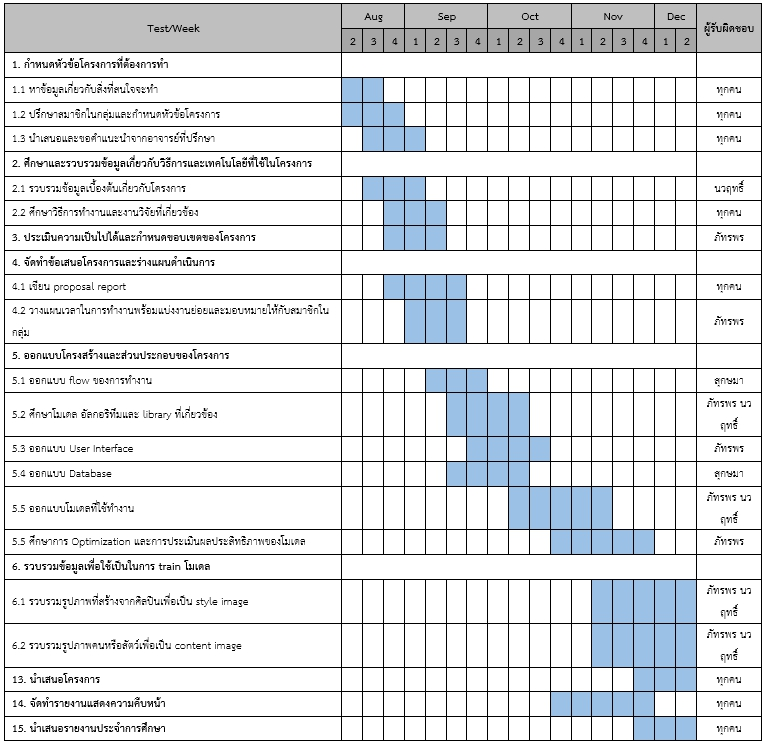
\includegraphics[width=15cm]{./image/plan_table1.jpg}
  \hfill
  \end{tabular}
\caption{ตารางแผนการทำงานภาคการศึกษาที่ 1\centering}
\label{tbl:symbols}
\end{table}

\newpage

\begin{table}[!h]
  \centering
  \begin{tabular}{c}
  \hfill
  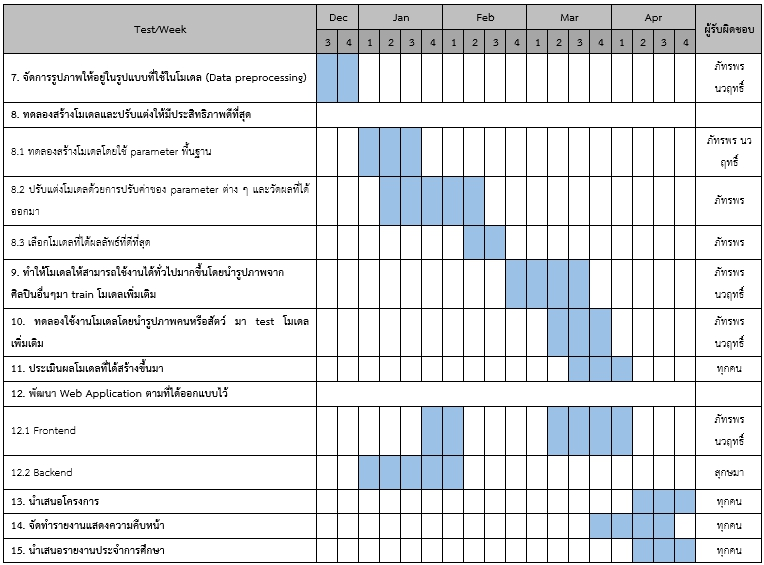
\includegraphics[width=15cm]{./image/plan_table2.jpg}
  \hfill
  \end{tabular}
\caption{ตารางแผนการทำงานภาคการศึกษาที่ 2\centering}
\label{tbl:symbols}
\end{table}


\section{ผลการดำเนินการ}
\subsection{ผลการดำเนินการในภาคการศึกษาที่1}
\begin{enumerate}
  \item ศึกษาและรวบรวมข้อมูลเกี่ยวกับวิธีการและเทคโนโลยีที่ใช้ในโครงการ
  \item ประเมินความเป็นไปได้และกำหนดขอบเขตของโครงการ
  \item จัดทำข้อเสนอโครงการและร่างแผนดำเนินการ
  \item ออกแบบโครงสร้างและส่วนประกอบของโครงการ
  \item รวบรวมข้อมูลเพื่อใช้เป็นในการ train โมเดล (style image และ content image)
  \item จัดการรูปภาพให้อยู่ในรูปแบบที่ใช้ในโมเดล (Data preprocessing)
  \item สร้างโมเดลโดยใช้ parameter พื้นฐาน
  \item จัดทำรายงานแสดงความคืบหน้า
\end{enumerate}

\newpage
\subsection{ผลการดำเนินการในภาคการศึกษาที่2}
\begin{enumerate}
  \item ทดลองสร้างโมเดลและปรับแต่งให้มีประสิทธิภาพดีที่สุด
  \item ทำโมเดลให้สามารถใช้งานได้ทั่วไปมากขึ้น
  \item ทดลองใช้งานโมเดล
  \item จัดทำ Web application ตามที่ออกแบบไว้
  \item นำเสนอโครงการ
  \item จัดทำรายงานแสดงความคืบหน้า
  \item นำเสนอรายงานประจำการศึกษา
\end{enumerate}


%%%%%%%%%%%%%%%%%%%%%%%%%%%%%%%%%%%%%%%%%%%%%%%%%%%%%%%%%%%%
%%%%%%%%%%%%%%  Literature Review %%%%%%%%%%%%%%%%%%%%%%%%%%
%%%%%%%%%%%%%%%%%%%%%%%%%%%%%%%%%%%%%%%%%%%%%%%%%%%%%%%%%%%%
\chapter{ทฤษฎีความรู้และงานที่เกี่ยวข้องงง}
\section{บทนำ}
\par\setlength{\parindent}{5ex}ในบทนี้ อธิบายเกี่ยวกับแนวคิดที่นำมาประยุกต์ใช้ในโครงงาน อัลกอริทึมที่ใช้ในการทำโครงงานคือ VGGNet และมีการพัฒนาโดยใช้ภาษา python นอกจากนี้มีการทบทวนวรรณกรรม ที่จะกล่าวถึงโครงงานที่มีลักษณะเนื้อหาที่เกี่ยวข้องกับการทำโครงการนี้

\section{แนวความคิดทางทฤษฎี}
\subsection{Neural style transfer}
\par\setlength{\parindent}{5ex}Neural Style Transfer [14] เป็นกระบวนการที่ใช้ CNNs ในการประมวลผลรูปภาพให้ได้รูปภาพที่เหมือนกับรูปภาพที่ใช้เป็น content image แต่มีรูปแบบหรือลักษณะที่ต่างกันไปตามรูปภาพที่ใช้เป็น style image ดังรูปที่ 2.1


\begin{figure}[!h]
  \centering
  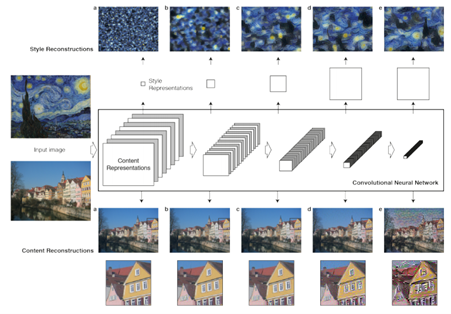
\includegraphics[width=15cm]{./image/unit1.png}
  \caption{แสดงหลักการทำงานของ Neural Style Transfer ที่ใช้ Convolutional Neural Network (CNN) }
  \label{fig:my_label}
  \source{Source of the image.}
\end{figure}

\section{อัลกอริทึมในการประมวลผลข้อความ}
\subsection{อัลกอริทึม I}

% Can define this in the preamble..
You can place the figure and refer to it as รูปที่~\ref{fig:model2}.
The figure and table numbering will be run and updated automatically when you add/remove tables/figures from the document.

\begin{figure}[!h]\centering
\setlength{\fboxrule}{0.2mm} % can define this in the preamble
\setlength{\fboxsep}{1cm}
\fbox{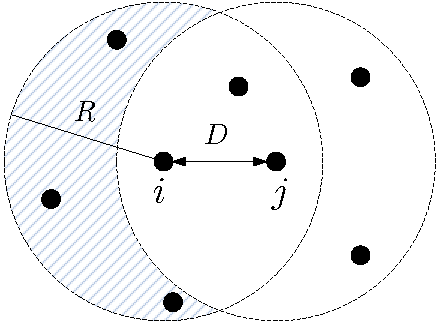
\includegraphics[width=5cm]{./model2.pdf}}
\caption{The network model}\label{fig:model2}
\end{figure}

 
\subsection{อัลกอริทึม I}
Add more subsections as you want.


\section{เครื่องมือที่ใช้ในการพัฒนา}

%%%%%%%%%%%%%%%%%%%%%%%%%%%%%%%%%%%%%%%%%%%%%%%%%%%%%55
%%%%%%%%%%%%%%%%%%%%%%%%%%%%%%%%%%%%%%%%%%%%%%%%%%%%%
%%%%%%%%%%%%%%%%%%%%%%%%%%%%%%%%%%%%%%%%%%%%%%%%%%%%%
\chapter{วิธีการดำเนินงาน}

Explain the design (how you plan to implement your work) of your project. Adjust the section titles below to suit the types of your work. Detailed physical design like circuits and source codes should be placed in the appendix.

\section{ข้อกำหนดและความต้องการของระบบ}

\section{สถาปัตยกรรมระบบ}

\begin{table}[!h]
\centering
\caption{test table x1}\label{tbl:symbols}
\begin{tabular}{@{}p{0.07\textwidth}|p{0.7\textwidth}p{0.1\textwidth}}\hline
\multicolumn{2}{l}{\textbf{SYMBOL}}  & \textbf{UNIT} \\ \hline 
$\alpha$ & Test variable\hfill & m$^2$ \\
$\lambda$ & Interarrival rate\hfill &  jobs/second\\
$\mu$ & Service rate\hfill & jobs/second \\ \hline
\end{tabular}
%\begin{tabular}{c|c} \hline
% $\alpha$ & $\beta$ \\ \hline
% $\delta$ & $\mu$ \\ \hline
%\end{tabular}
\end{table}



\section{Hardware Module 1}
\subsection{Component 1}
\subsection{Logical Circuit Diagram}

\section{Hardware Module 2}
\subsection{Component 1}
\subsection{Component 2}

\section{Path Finding Algorithm}

\section{Database Design}

\section{UML Design}

\section{GUI Design}

\section{การออกแบบการทดลอง}
\subsection{ตัวชี้วัดและปัจจัยที่ศึกษา}
\subsection{รูปแบบการเก็บข้อมูล}




%%%%%%%%%%%%%%%%%%%%%%%%%%%%%%%%%%%%%%%%%%%%%%%%%%%%%%%%%%%%%%
%%%%%%%%%%%%%%%%%%%% Experiments %%%%%%%%%%%%%%%%%%%%%%%%%%%%%
%%%%%%%%%%%%%%%%%%%%%%%%%%%%%%%%%%%%%%%%%%%%%%%%%%%%%%%%%%%%%%%
\chapter{ผลการดำเนินงาน}

You can title this chapter as \textbf{Preliminary Results} ผลการดำเนินงานเบื้องต้น or \textbf{Work Progress} ความก้าวหน้าโครงงาน for the progress reports. Present implementation or experimental results here and discuss them.
ใส่เฉพาะหัวข้อที่เกี่ยวข้องกับงานที่ทำ 

\section{ประสิทฺธิภาพการทำงานของระบบ} 
\section{ความพึงพอใจการใช้งาน}
\section{การวิเคราะห์ข้อมูลและผลการทดลอง}

%%%%%%%%%%%%%%%%%%%%%%%%%%%%%%%%%%%%%%%%%%%%%%%%%%%%%%%%%%%%%%%
%%%%%%%%%%%%%%%%%%%% Conclusions %%%%%%%%%%%%%%%%%%%%%%%%%%%%%
%%%%%%%%%%%%%%%%%%%%%%%%%%%%%%%%%%%%%%%%%%%%%%%%%%%%%%%%%%%%%%%
\chapter{บทสรุป}

This chapter is optional for proposal and progress reports but 
is required for the final report.

\section{สรุปผลโครงงาน}
สรุปว่าโครงงานบรรลุตามวัตถุประสงค์ที่ตั้งไว้หรือไม่ อย่างไร 

\section{ปัญหาที่พบและการแก้ไข}
State your problems and how you fixed them.

\section{ข้อจำกัดและข้อเสนอแนะ}
ข้อจำกัดของโครงงาน What could be done in the future to make your projects better.

%%%%%%%%%%%%%%%%%%%%%%%%%%%%%%%%%%%%%%%%%%%%%%%%%%%%%%%%%%%%%%%
%%%%%%%%%%%%%%%%%%%% Bibliography %%%%%%%%%%%%%%%%%%%%%%%%%%%%%
%%%%%%%%%%%%%%%%%%%%%%%%%%%%%%%%%%%%%%%%%%%%%%%%%%%%%%%%%%%%%%%

%%%% Comment this in your report to show only references you have
%%%% cited. Otherwise, all the references below will be shown.
\nocite{*}
%% Use the kmutt.bst for bibtex bibliography style 
%% You must have cpe.bib and string.bib in your current directory.
%% You may go to file .bbl to manually edit the bib items.
\bibliographystyle{kmutt}
\bibliography{string,cpe}

%%%%%%%%%%%%%%%%%%%%%%%%%%%%%%%%%%%%%%%%%%%%%%%%%%%%%%%%%%%%%%%
%%%%%%%%%%%%%%%%%%%%%%%% Appendix %%%%%%%%%%%%%%%%%%%%%%%%%%%%%
%%%%%%%%%%%%%%%%%%%%%%%%%%%%%%%%%%%%%%%%%%%%%%%%%%%%%%%%%%%%%%%
\appendix{ชื่อภาคผนวกที่ 1}
\noindent{\large\bf ใส่หัวข้อตามความเหมาะสม} \\

This is where you put hardware circuit diagrams, detailed experimental data in tables or source codes, etc.. \\ \bigskip



This appendix describes two static allocation methods for fGn (or fBm)
traffic. Here, $\lambda$ and $C$ are respectively the traffic arrival
rate and the service rate per dimensionless time step. Their unit are
converted to a physical time unit by multiplying the step size
$\Delta$. For a fBm self-similar traffic source,
Norros~\cite{norros95} provides its EB as
\begin{equation}\label{eq:norros}
  C = \lambda + (\kappa(H)\sqrt{-2\ln\epsilon})^{1/H}a^{1/(2H)}x^{-(1-H)/H}\lambda^{1/(2H)}
\end{equation}
where $\kappa(H) = H^H(1-H)^{(1-H)}$. Simplicity in the calculation is
the attractive feature of (\ref{eq:norros}).

The MVA technique developed in~\cite{kim01} so far provides the most
accurate estimation of the loss probability compared to previous
bandwidth allocation techniques according to simulation results.
Consider a discrete-time queueing system with constant service rate
$C$ and input process $\lambda_n$ with $\mathbb{E}\{\lambda_n\} =
\lambda$ and $\mathrm{Var}\{\lambda_n\} = \sigma^2$.  Define $X_n \equiv
\sum_{k=1}^n \lambda_k - Cn$.  The loss probability due to the MVA
approach is given by
\begin{equation}\label{eq:loss_mva}
  \varepsilon \approx \alpha e^{-m_x/2}
\end{equation}
where
\begin{equation}\label{eq:mx}
m_x = \min_{n \geq 0} \frac{((C-\lambda)n + B)^2}{\mathrm{Var}\{X_n\}} =
\frac{((C-\lambda)n^\ast + B)^2}{\mathrm{Var}\{X_{n^{\ast}}\}}
\end{equation} 
and 
\begin{equation}\label{eq:alpha}
  \alpha =
  \frac{1}{\lambda\sqrt{2\pi\sigma^2}}\exp\left(\frac{(C-\lambda)^2}{2\sigma^2}\right)
  \int_C^\infty (r-C)\exp\left(\frac{(r-\lambda)^2}{2\sigma^2}\right)\, dr
\end{equation}
For a given $\varepsilon$, we numerically solve for $C$ that satisfies
(\ref{eq:loss_mva}). Any search algorithm can be used to do the task.
Here, the bisection method is used.  

Next, we show how $\mathrm{Var}\{X_n\}$ can be determined.  Let
$C_{\lambda}(l)$ be the autocovariance function of $\lambda_n$.  The
MVA technique basically approximates the input process $\lambda_n$
with a Gaussian process, which allows $\mathrm{Var}\{X_n\}$ to be
represented by the autocovariance function.  In particular, the
variance of $X_n$ can be expressed in terms of $C_{\lambda}(l)$ as
\begin{equation}
  \mathrm{Var}\{X_n\} = nC_{\lambda}(0) + 2\sum_{l=1}^{n-1} (n-l)C_{\lambda}(l)
\end{equation} 
Therefore, $C_{\lambda}(l)$ must be known in the MVA technique, either
by assuming specific traffic models or by off-line analysis in case of
traces.  In most practical situations, $C_{\lambda}(l)$ will not be
known in advance, and an on-line measurement algorithm developed
in~\cite{eun01} is required to jointly determine both $n^\ast$ and
$m_x$. For fGn traffic, $\mathrm{Var}\{X_n\}$ is equal to $\sigma^2
n^{2H}$, where $\sigma^2 = \mathrm{Var}\{\lambda_n\}$, and we can find
the $n^\ast$ that minimizes (\ref{eq:mx}) directly. Although $\lambda$
can be easily measured, it is not the case for $\sigma^2$ and $H$.
Consequently, the MVA technique suffers from the need of prior
knowledge traffic parameters.


%%%%%%%%%%%%%%%%%%%%%%%%%%%%%%%%%%%%%%%%%%%%%%%%%%%%%%%%%%
%%%%%%%%%%%%%%% The 2nd appendix %%%%%%%%%%%%%%%%%%%%%%%%%%
%%%%%%%%%%%%%%%%%%%%%%%%%%%%%%%%%%%%%%%%%%%%%%%%%%%%%%%%%%
\appendix{ชื่อภาคผนวกที่ 2}
\noindent{\large\bf ใส่หัวข้อตามความเหมาะสม} \\

Next, we show how $\mathrm{Var}\{X_n\}$ can be determined.  Let
$C_{\lambda}(l)$ be the autocovariance function of $\lambda_n$.  The
MVA technique basically approximates the input process $\lambda_n$
with a Gaussian process, which allows $\mathrm{Var}\{X_n\}$ to be
represented by the autocovariance function.  In particular, the
variance of $X_n$ can be expressed in terms of $C_{\lambda}(l)$ as
\begin{equation}
  \mathrm{Var}\{X_n\} = nC_{\lambda}(0) + 2\sum_{l=1}^{n-1} (n-l)C_{\lambda}(l)
\end{equation} 

\noindent{\large\bf Add more topic as you need} \\

Therefore, $C_{\lambda}(l)$ must be known in the MVA technique, either
by assuming specific traffic models or by off-line analysis in case of
traces.  In most practical situations, $C_{\lambda}(l)$ will not be
known in advance, and an on-line measurement algorithm developed
in~\cite{eun01} is required to jointly determine both $n^\ast$ and
$m_x$. For fGn traffic, $\mathrm{Var}\{X_n\}$ is equal to $\sigma^2
n^{2H}$, where $\sigma^2 = \mathrm{Var}\{\lambda_n\}$, and we can find
the $n^\ast$ that minimizes (\ref{eq:mx}) directly. Although $\lambda$
can be easily measured, it is not the case for $\sigma^2$ and $H$.
Consequently, the MVA technique suffers from the need of prior
knowledge traffic parameters. 





\end{document}
